\Gls{ML} is a sub-field of \gls{AI} within the broad category of
computer science. The goal of \gls{AI} is to create computer systems that
respond to their environment according to some set of criteria or goal
\cite{changingml}.  For example, self-driving vehicles have computers on board
that learn to avoid curbs and humans. While its use has been increasing in the
commercial sector, there is also much anecdotal evidence to support the
existence of a rapid increase of \gls{AI} use in academic research across many
disciplines beyond robotics. \gls{AI} systems have been used in detection
(e.g., fraud or spam), medical diagnostics, user analysis (e.g., Netflix
ratings), and a host of scientific disciplines that have increasing amounts of
multivariate data.

\gls{ML} research focuses on the underlying algorithms using mathematical
optimization, methods for pattern recognition, and computational statistics.
Much of the recent advances to the field of \gls{AI} have occurred in the
statistical realm, which forgoes domain knowledge in favor of large data sets.
In this work, there is no distinction made between the terminology of machine
learning and statistics.  Additionally, this study is not concerned with
computational time, but rather the ability to correctly predict values and
categories relevant to the nuclear forensics mission. This restricts the
relevancy of the algorithms to the underlying theory and its impact on the
resulting model's accuracy. 

\gls{ML} algorithms can be separated into two main categories: unsupervised and
supervised learning.  The former groups or interprets a set of input data,
predicting patterns or structures. The latter includes both the input and
output data, enabling the \gls{ML} model to predict future outputs.  Broadly
speaking, the unsupervised learning algorithms are designed for clustering data
sets or dimensionality reduction (i.e., determining some subset or linear
combination of features most relevant to the input data) of data sets.
Supervised learning algorithms predict both discrete and continuous values via
classification and regression, respectively. Some algorithms can perform both
classification and regression, and neural networks can even be modified to
perform either supervised or unsupervised learning.\cite{elements_stats} 

\begin{figure}[!htb]
  \makebox[\textwidth][c]{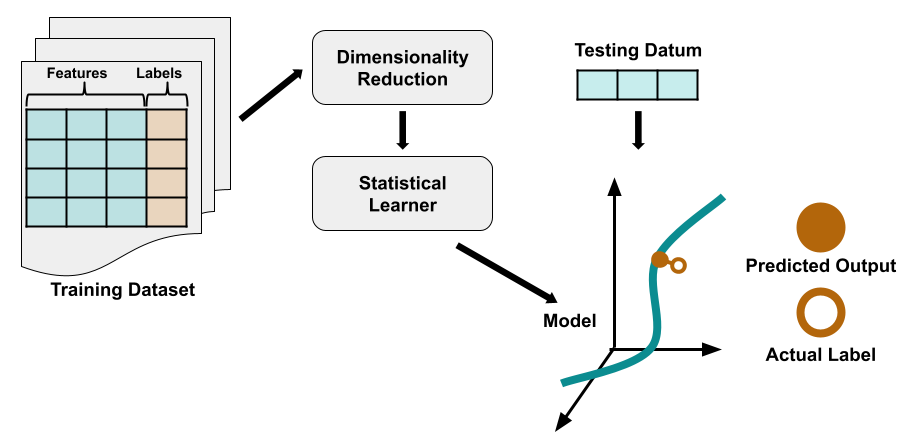
\includegraphics[width=\textwidth]{./chapters/litrev/SupervisedRegression.png}}
  \caption{Diagram of a supervised machine learning process: a model 
           created from a training data set and a statistical learner (with
           an optional dimensionality reduction step) allows a prediction
           when introduced with a test sample. If the actual label is known,
           an error in model performance can be calculated.}
  \label{fig:supervised}
\end{figure}

As shown in Figure \ref{fig:supervised}, a typical (supervised) machine
learning workflow begins with a training data set, which has a number of
\textit{instances}, or rows of \textit{observations}.\todo{check language from later on; I think I use entries and samples a lot}  Each instance has some
\textit{attributes}, also referred to as \textit{features}. It also has a
\textit{label}, which can be a categorical label or discrete/continuous values.  

The training data are then inserted into a statistical learner, where the
learner is capable of predicting labels given a set of features. The algorithm
for the statistical learner calculates some objective, minimizes or maximizes
that objective, and provides some model.  This model can be evaluated using a
testing set that has the same set of features and labels (but different
observations). The comparison of what the model predicts and the actual label
gives the \textit{testing error}.  Depending on the performance and
application, the model may need improvement from more training and/or some
changes in the algorithm parameters. Once the model is performing well enough
and validated, it is finalized; then a user can provide a single observation
and a value can be predicted from that. 

This study performs regression tasks using supervised learning algorithms.
Differences among the structure underlying mathematics of the algorithms impact the
\gls{ML} models.  Therefore, the algorithms used in this study will be discussed
in Section \ref{sec:algs}. Next, a discussion on model performance and prediction 
errors takes place in Section \ref{sec:errs}.

\subsection{Algorithms for Statistical Learning}
\label{sec:algs}
%\setlength\abovedisplayskip{2.5pt}

For relevant nuclear forensics predictions, both classification and regression
algorithms must be used.  For example, one may want to predict the reactor type
label given some measurement-based features of \gls{SNF} of an unknown source.
This would require a classification algorithm. Or perhaps the input fuel
composition is relevant to an investigation on weapons intent, so a regression
algorithm would be used. 

There are three algorithms presented in this section: \textit{k}-nearest
neighbors, decision trees, and \gls{MLL} calculations. They were chosen based
on their simplicity; this work has yet to be benchmarked using simple
algorithms so a more complex treatment of the training sets in this work would
be premature. Additionally, in part because of their simplicity, they are all
"white box" methods.  This is unique in the \gls{ML} universe, since most
algorithms create a black box model that is unable to be analyzed by a human.
The  decision trees method provides an output model that can be used to discern
behavior and understand predictions, and \textit{k}-nearest neighbors and
\gls{MLL} calculations do not create a model at all. Individual predictions can
still be analyzed, however, since the procedures are so simple. 

\subsubsection{Nearest Neighbor Methods}

Nearest neighbors classification and regression are unique algorithms in
that thay are instance-based; they do not actually generalize, but instead
track the observations in the training set.  The main metric for this algorithm
is distance (or dissimilarity) between the test sample and the closest training
sample(s) in the vicinity.  During prediction, the algorithm will calculate a
value based on the instance that is closest to the current test sample. Thus,
there is not any learning, but instead a direct comparison between an unknown
sample and the space that the training set populates. The predictions from
nearest neighbors can be quite accurate, but are highly unstable to
peturbations \cite{elements_stats}.

The process of prediction with \textit{k}-nearest neighbors is as follows.
First, the distances between the test sample and each of the training set
instances are calculated.  Most commonly the Euclidian distance is used, but
this walkthrough uses the Manhattan distance:
\begin{equation}
  d_{i} = \sum_{j=1}^{N_{feats}} |x_{j,train} - x_{j,test}|
  \label{eq:l1}
\end{equation}
where $i$ is each training set instance, and $j$ refers to each feature in the
training set.  The lowest \textit{k} $d_{i}$ are chosen. For \textit{k}-nearest
neighbors regression, the value, $y$ is predicted using the following equation.
\begin{equation}
  y(\boldsymbol{x}) = \frac{1}{k} \sum_{i=1}^{k} w_i \cdot y_i
  \label{eq:knn}
\end{equation}
where $w_{i}$ is either uniform and takes on a value of $1$ or is
distance-based and takes on a value of $1/d_{i}$ and $\boldsymbol{x}$ is the
full set of features. The regression equation averages the closest \textit{k}
neighbors for an estimate of the unknown sample.  In \textit{k}-nearest
neighbors classification, the class label $y$ is predicted using the mode of
the nearest neighbors selected using the \textit{k} smallest $d_i$, or when
$w_i$ is $1/d{i}$ the weighted mode is used to choose the predicted label.

\begin{figure}[!htb]
  \centering
  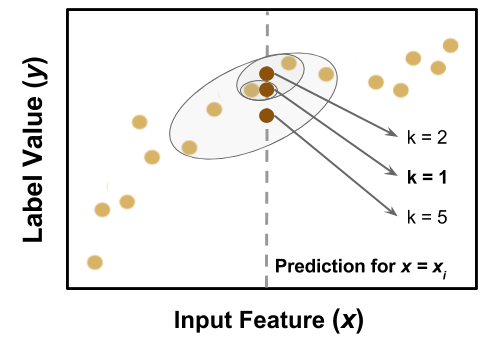
\includegraphics[width=0.8\linewidth]{./chapters/litrev/nn-fig.png}
  \caption{Schematic of \textit{k}-nearest neighbors regression, showing how 
           changing \textit{k} alters the predicted label value $y$.}
  \label{fig:nn}
\end{figure}

Figure \ref{fig:nn} provides a pictoral explanation of Equation \ref{eq:knn}
for a prediction where there is one feature. In this figure, there is a test
sample with a feature, valued at $x_i$, indicated with the grey dotted line.
The three circles represent the neighborhood given by the value of \textit{k},
and the darker dots on the line represent the reported prediction $y$ for each
choice of \textit{k}.  In this illustration, $k=1$ or $k=2$ provide a more
accurate prediction according to a visual inspection of the trend, but higher
values of $k$ can be useful, and will be discussed in Section
\ref{sec:complexity}.

\subsubsection{Decision Trees}

Decision trees are a common choice because they are simple to implement and
provide an interpretable model. However, the predictions from decision trees,
similar to \textit{k}-nearest neighbors, are unstable to peturbations.  What
follows is a highly simplified explanation of the Classification and Regression
Trees algorithm for growing decision trees, showing only the equations for
splitting criteria.  A more complete treatment can be found in Reference
\cite{elements_stats} or in the User Guide in Reference \cite{scikit}.

At their core, decision trees algorithms split the feature space into different
regions.  Decision trees are constructed by iteratively finding places in the
feature space at which to split the data to best predict a label. Some measure
of information gain (more accurately the opposite, impurity, denoted here as
$H$) is used to select a splitting criterion at each split, which maximizes
differentiation between average label values in regression or groups similar
labels together in classification.  This process continues until some
externally set stopping requirement is met, or no information gain can be made
by continuing to create splits. 

Each split creates two new nodes on the tree, where the node has to find a new
splitting criterion. In the math that follows, there are nodes given by $m$,
and a number of samples in each node given by $N_{\text{samples}, m}$. The
individual node samples are given by $i$. The impurity at the node is denoted
as $H(m)$. In classification, the node impurity can be measured by the Gini
index, where $p_{m, k}$ is the proportion of class $k$ observations at the
node:
\begin{equation}
  \begin{aligned}
    p_{m, k} &= \frac{1}{N_{\text{samples}, m}} \sum_{i=1}^{N_{\text{samples}, m}}
              I(y = k)
    \\
    H(m) &= \sum_k p_{m, k} (1 - p_{m, k})
  \end{aligned}
\end{equation}
And in regression, the node impurity $H(m)$ can be measured by the mean squared
error, where $\bar{y}_m$ is the average value of the samples in the node.
\begin{equation}
  \begin{aligned}
    \bar{y}_m &= \frac{1}{N_{\text{samples}, m}} \sum_{i=1}^{N_{\text{samples}, m}} 
                 y_{i, m}
    \\
    H(m) &= \frac{1}{N_{\text{samples}, m}} \sum_{i=1}^{N_{\text{samples}, m}}
              (y_i - \bar{y}_{i, m})^2
  \end{aligned}
\end{equation}
The splitting criterion with the lowest impurity is the one that is chosen to
make the split.  This will partition the feature space and the splitting
process will continue until a pre-defined tree size or number of samples per
node. Without a pre-defined stopping point the tree will grow until there is
one sample per node. This process can be understood more intuitively by
stuyding Figure \ref{fig:dtr}. Note that this tree was created using a maximum
tree depth of $2$ for visualization purposes in order to explain the process,
so is not indicative of a real decision tree.

\begin{figure}[!htb]
  \centering
  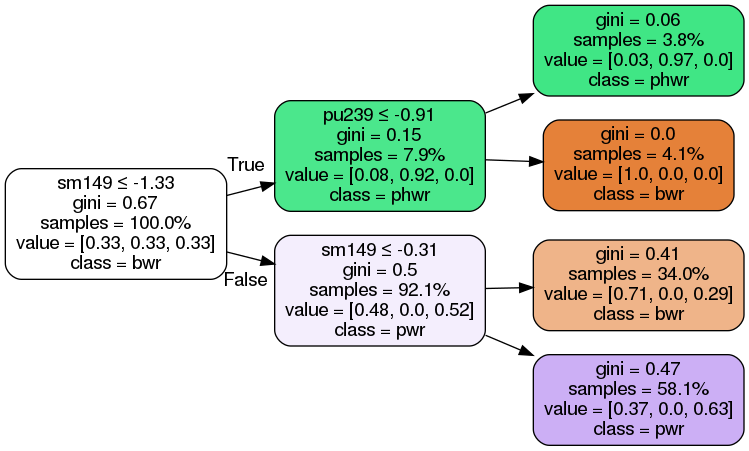
\includegraphics[width=\linewidth]{./chapters/litrev/dtree.png}
  \caption{Example of a decision tree process, where maximum tree depth was 
           limited to 2 for vizualization purposes.}
  \label{fig:dtr}
\end{figure}

In Figure \ref{fig:dtr}, the first split is determined to occur at the feature
Sm149 on whether the nuclide measurement is above a value of $-1.33$. Note that
this value is negative because of the scaling process the training set is put
through, described in Section \ref{sec:statmodel1}. The majority class at this
node is \gls{BWR} which is expected since the training set is 72\% \gls{BWR}.
The values list indicates the fraction of each class in the node, which is
alphabetically ordered \texttt{[bwr, phwr, pwr]}. It is even among the three
because the class weights were told to be balanced.  This splitting criterion
provides a Gini impurity score of 0.67, which represents the minimum Gini
impurity of all the candidate splits, but also indicates there are multiple
classes represented in this node (again, expected).  It would be 0 if there
were only one class in the node.  In the visualization, the shading of the
colors in the tree are bolder for there being a higher fraction of a single
class.

\subsubsection{Maximum Log-Likelihood Calculations}

The \gls{MLL} calulations approach applied here is based on a method developed
to do similar work \cite{mll_method, mll_validate, mll_sensitivity}.  That work
involved matching nuclear material samples based on some select measurements to
entries in a database of containing those measurements (see Section
\ref{sec:stats4nf}).  Each database entry also has a similar list of labels to
the labels being predicted in this work: reactor type, burnup, and time since
irradiation.

Interestingly, the \gls{MLL} calculations method works like \textit{k}-nearest
neighbors, where there is no model but a prediction according to the closest
match database entry.  There is one detail that differs, however. Whereas
\textit{k}-nearest neighbors minimizes distance/dissimilarity, this approach
instead maximizes similarity via a likelihood function. An "unknown" test
sample is compared against the training set using the likelihood calculation
between that sample and the training set entries.  The higher the likelihood,
the higher the probability that the database entry represents the sample. The
likelihood is in Equation \ref{eq:like}, whereas the log-likelihood is used
more often in practice, shown in Equation \ref{eq:loglike}.
\begin{equation}
  L(M|x_{test}) = \prod_i \frac{1}{\sigma_{i,train} \sqrt{2\pi}} \exp{\frac{-(x_{i,test} - x_{i,train})^2}{2 \sigma_{i,train}^2}}
  \label{eq:like}
\end{equation}
\begin{equation}
  ln(L(M|x_{test})) = \sum_i ln(\frac{1}{\sigma_{i,train} \sqrt{2\pi}}) - \frac{(x_{i,test} - x_{i,train})^2}{2 \sigma_{i,train}^2}
  \label{eq:loglike}
\end{equation}
The likelihood is a measure of the probability that a model $M$ produced the
measurements seen in the test sample, given by $L(M|x_{test})$.  In both
Equations \ref{eq:like} and \ref{eq:loglike}, $x$ refers to the set of
features, and $x_{i, test}$ and $x_{i,train}$ are the individual features for the
test sample and the training set entries, respectively. The uncertainty of the
measurement associated with each feature is represented by $\sigma_{i,train}$.



\subsection{Algorithm Performance}
\label{sec:errs}
After a model is trained, its performance must be evaluated. The following
discusses the considerations taken for the evaluation of the prediction
performance for the algorithms used in this work. 

\gls{ML} algorithms are heavily dependent on the training inputs and algorithm
parameters given to them, such as training set sizes, regularization (defined
below in Section \ref{sec:complexity}), number of features in the training set,
algorithm hyperparameters, etc.  To obtain reliable models, one must both
choose or create a training set carefully and study the impact of various
algorithm parameters on the error. Various error metrics are first covered in
Section \ref{sec:testerr} before the causes of error are discussed in Section
\ref{sec:complexity}.

\subsubsection{Testing Error}
\label{sec:testerr}

The creation of an \gls{ML} model is (usually) a hidden process. Although the
model emerges from a black box, there are ways to evaluate its generalization
(i.e., prediction) capability.  This is done by removing a small portion of the
database for use as a testing set.  The rest of the data set is known as the
training set and is used to train a model. After training, the test set is used
to calculate the model's error to unseen test samples.  This error is typically
referred to as the \textit{testing error}, as it is measuring the ability of
the model to predict future cases that were not introduced in the training
phase. Next, the various metrics used to evaluate classification and regression
are covered.

%In addition to evaluating a single learned model, it is beneficial to compare
%models. Moreover, there are potential degeneracies in the solution space. This
%is because most inverse problems are \textit{ill-posed}, because the solution
%is not guaranteed to be unique \cite{skutnik_2016}.  Evaluating not only the
%solution, but the confidence in the solution, is therefore prudent. While the
%two scikit-implemented algorithms do not provide this information, the
%\gls{MLL} calculation method provides a likelihood with an uncertainty. This
%provides a measure of distinguishability that many machine learning approaches
%do not provide. 

\noindent \textbf{Reactor Type Classification}

For the classification of reactor type, it is typical to use an accuracy score
for classification, where the total number of correct predictions is taken as a
fraction of the entire sample set.
\begin{equation}
  \textit{accuracy} = \frac{1}{N_\text{samples}} \sum_{i=1}^{N_\text{samples}} 
                      \mathbb{I}(y_{pred,i} = y_{true,i})
\end{equation}
Note that $\mathbb{I}(x)$ here is being used to refer to the indicator
function, where when $x$ is true it takes a value of 1 and when $x$ is false it
takes a value of 0.

But training sets can have an uneven number of classes represented.  A more
fair scoring system for imbalanced data sets is instead balanced accuracy,
which averages the accuracy of each class. This would provide a range from 0 to
1. In this work, however, the balanced accuracy is used with
\texttt{adjusted=True} in scikit-learn. This rescales the range to
$\frac{1}{1-N_\text{classes}}$ to 1, where 0 is considered random scoring.
This is done by defining a sample weight as the following, based on its class
frequency $w_j$ \cite{scikit}. This differs from the definition in the
scikit-learn documentation because it presumes a previous sample weight,
whereas this work does not pre-define sample weights.
\begin{equation}
  w_i = \frac{1}{\sum_j{\mathbb{I}(y_j = y_i) w_j}}
\end{equation}
for \textit{j} classes and \textit{i} samples. Thus, the balanced accuracy is
the following with the adjusted weights.
\begin{equation}
  \textit{balanced-accuracy} = \frac{1}{\sum_{i}{w_i}} \sum_{i=1}^{N_\text{samples}}
                               w_i \cdot \mathbb{I}(y_{pred, i} = y_{true_i})
\end{equation}

\begin{figure}[!htb]
  \centering
  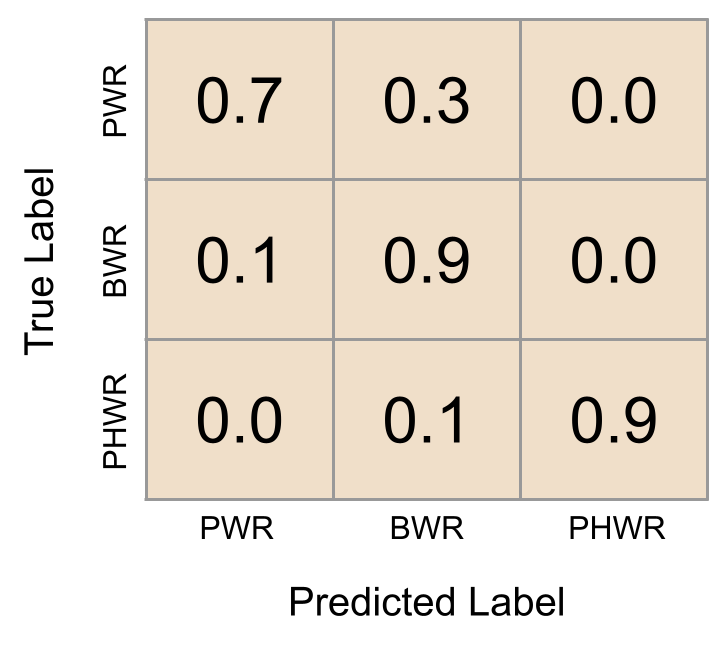
\includegraphics[width=0.4\linewidth]{./chapters/litrev/cm_example.png}
  \caption[Example of a confusion matrix]
          {Example of a confusion matrix for the three reactor types}
  \label{fig:cm_ex}
\end{figure}

In addition to the metrics which combine the knowledge of true positive and
true negative predictions, it is also important to study the
misclassifications. Confusion matrices show both the true positive predictions
and the false positive predictions, which can be useful information in
understanding an imperfect accuracy or balanced accuracy score. For example,
Figure \ref{fig:cm_ex} pictures an example confusion matrix that could result
from this data set, where a fraction of \glspl{PHWR} are correctly predicted
(0.9), but there are some misclassified as \gls{BWR} (0.1).  While there are no
\glspl{PWR} or \glspl{BWR} misclassified as \gls{PHWR}, they do get
misclassified as each other: 0.3 \glspl{PWR} and 0.1 \glspl{BWR} get
misclassified as the other.  Note that each row must add up to 1, since those
are the true class labels. The columns do not add up to 1 (unless there are no
misclassifications).  

\noindent \textbf{Regression Mean Error Calculations}

For the three regression cases, there are a few metrics that are being
calculated to measure prediction performance: the \gls{MAE}, \gls{MedAE}, and
\gls{MAPE}. The most common metrics to use for comparing regression errors are
\gls{RMSE} or \gls{MAE}, but these mean errors do not provide the full picture.
The \gls{MedAE} can provide interesting insight into a middle-ground or
majority behavior. Also, the relative error via \gls{MAPE} can provide insight
especially when there is a large span of values for a regression case; a large
absolute error could be a small relative error. Therefore, they are all
tracked.  The \gls{MAE}, \gls{MedAE}, and \gls{MAPE} are calculated as follows,
respectively, for each label $j$ (which is suppressed in the math below for
clarity).
\begin{equation}
  \textit{MAE} = \frac{1}{N_{\text{samples}}} \sum_{i=1}^{N_{\text{samples}}} 
                 \left| y_{true, i} - y_{pred, i} \right|
\end{equation}
\begin{equation}
  \textit{MedAE} = \text{median}(\mid y_{true, 1} - y_{pred, 1} \mid, \ldots, 
                                 \mid y_{true, n} - y_{pred, n} \mid)
\end{equation}
\begin{equation}
  \textit{MAPE} =  \frac{100}{N_{\text{samples}}} \cdot 
                   \sum_{i=1}^{N_{\text{samples}}}
                   \frac{\left| y_{true, i} - y_{pred, i} \right|}{y_{true, i}}
\end{equation}

\noindent \textbf{Cross Validation}

A testing set that would be used during training to give feedback, a
\textit{\gls{CV} set}, can provide a faster convergence to a satisfactory
model. As shown in Figure \ref{fig:cverror}, this can be done by splitting the
data set into three groups: a large training set, a small \gls{CV} set, and a
small testing set.  

\begin{figure}[!htb]
  \centering
  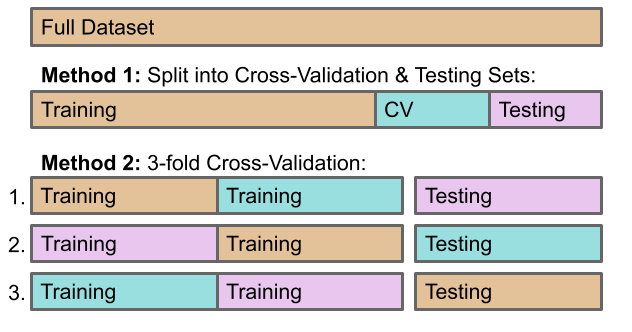
\includegraphics[width=0.85\linewidth]{./chapters/litrev/cverror.png}
  \caption[Illustration of cross validation]
          {Illustration of two ways of performing \gls{CV}: a one-time split, 
           or \textit{k}-fold \gls{CV}.}
  \label{fig:cverror}
\end{figure}

However, in practice, multiple rounds of \gls{CV} steps are used provide a
better estimate of model performance by increasing the number of testing sets.
This is referred to as \textit{k-fold cross-validation}.  An example where
$k=3$ is illustrated in Figure \ref{fig:cverror}.  One partition of the
training set is designated as the testing set, and a model is trained with the
rest. This returns the testing error for that first testing partition.
Following the first training phase, another begins, this time with a different
subset as the testing set.  In total, this process is performed three times,
giving three models. Since each partition becomes a testing set at one point,
all entries in the training set are tested, which reduces the chance that the
model is being tested with a misrepresentative testing set. In most
applications, the testing error results from each partition (which are an
average of all test cases in that partition) are averaged to provide a picture
of the model performance. However, this work instead focuses on the aggregate
statistics of all the \textit{individual} test case errors taken together,
regardless of which partition they were in.

\subsubsection{Model Complexity}
\label{sec:complexity}

In statistical learning, there are two sources of error that need to be
simultaneously minimized: bias and variance. Bias is caused by simplifications
in the model, so the error is caused by missed relationships in the data; high
bias is an indication of an underfit model.  Variance is caused by including
random noise in the model, so the error is caused by oversensitivity to that
noise; high variance is an indication of an overfit model. What follows is a
discussion on error considerations that all reduce to one concept: how
\textit{complex should a model be} to best predict a previously unseen test
sample?

\begin{figure}[!htb]
  \makebox[\textwidth][c]{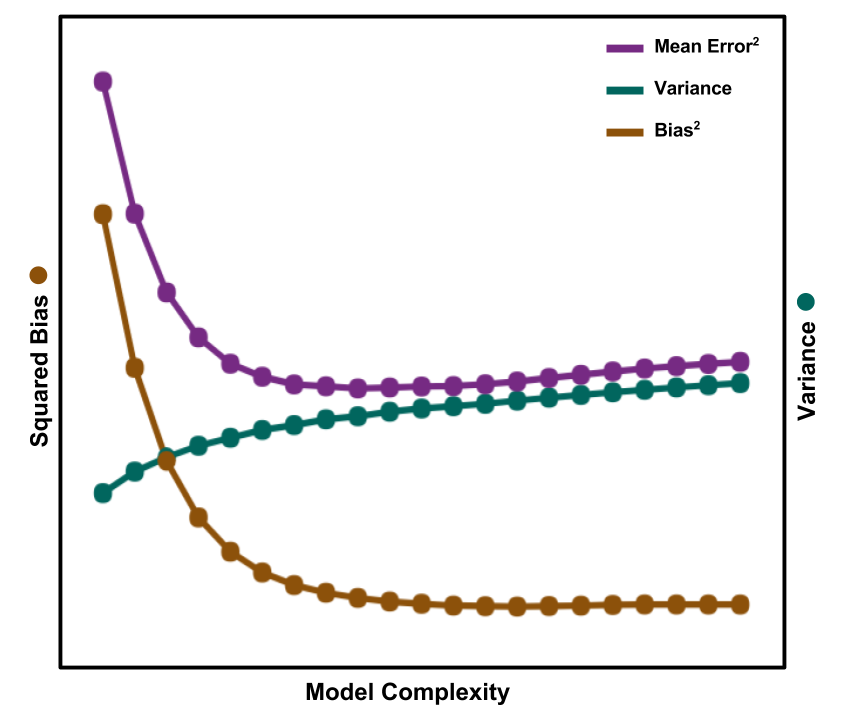
\includegraphics[width=0.7\textwidth]{./chapters/litrev/BVtradeoff.png}}
  \caption[Schematic of the bias-variance trade-off]
          {Schematic showing the sources of error, bias and variance, and how 
           they behave with respect to model complexity in the bias-variance 
           trade-off.}
  \label{fig:bvtradeoff}
\end{figure}

Figure \ref{fig:bvtradeoff} shows the tradeoff between the bias and variance.
The shape of the total error curve has a minimum that we seek to achieve with
our model. Some bias is desired in order to generalize to future unknown data.
But, some variance is positive for the model because it captures the
relationships in the data that the bias counteracts. 

\textit{Regularization} refers to introducing a term into the \gls{ML} model to
prevent overfitting; it is used in many \gls{ML} algorithms to reduce the model
complexity and therefore the resulting variance.  This would be represented by
increasing \textit{k} in \textit{k}-nearest neighbors, or reducing the maximum
features a decision trees implementation could consider for splitting.  The top
three windows in Figure \ref{fig:complex} show the effects of regularization on
a simple linear regression model. With heavy regularization comes high bias,
represented by the left-most window.  The right-most window shows a low
regularization scenario, where most individual points are tracked by the model,
but generalizing beyond that might be problematic. The middle plot represents an 
approximately well-fit model.  

\begin{figure}[!htb]
  \centering
  \makebox[\textwidth][c]{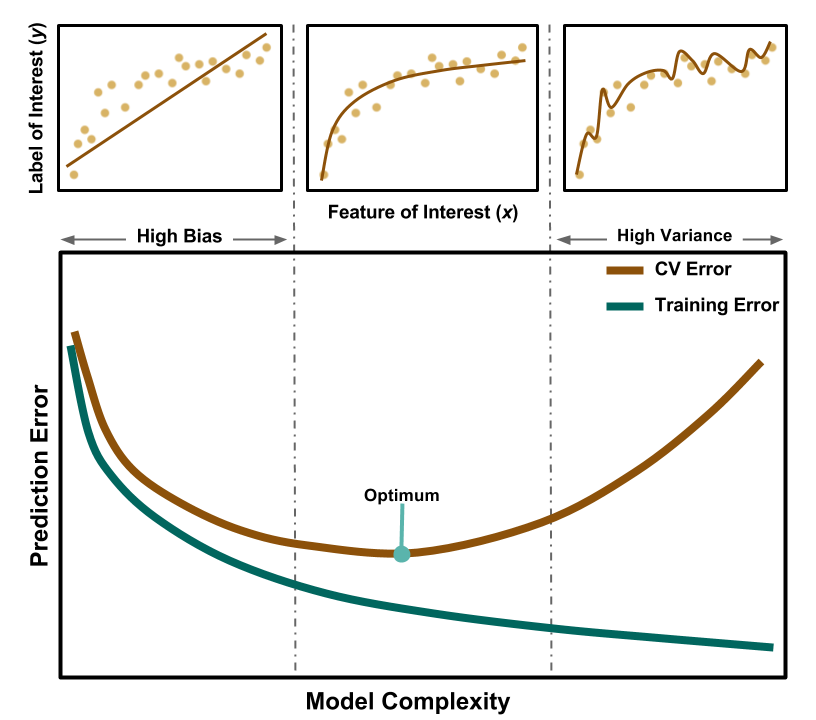
\includegraphics[width=0.9\textwidth]{./chapters/litrev/ValidationCurve.png}}
  \caption[Diagram of model performance with respect to model complexity]
          {Diagram showing effect of model complexity/regularization at three 
           different levels on model performance.}
  \label{fig:complex}
\end{figure}

Diagnostic plots show the testing errors with respect to some variable on the
\textit{x}-axis.  Typically this variable is related in some way to the model
complexity. This provides insight into the model's fitness, and whether small
tweaks can be made to increase bias or variance to improve testing performance.
Put another way, these approaches can evaluate under- or over-fitting.  When
the \textit{x}-axis is related to regularization parameters, often referred to
as algorithm hyperparameters in this work, it is known as a \textit{validation
curve}. A full treatment of validation curves is not considered here, but
Figure \ref{fig:complex} shows the portion relevant to the discussion in the
bottom plot.  The negative prediction error is plotted on the \textit{y}-axis
so that the orientation of higher is better is maintained.  A parameter
influencing model complexity is on the \textit{x}-axis.  The testing error is
typically low for the high bias and high variance models, but there usually
exists an optimum parameter for model complexity for most training data sets. 

Another parameter indirectly influencing model complexity is the training set
size.  When the training set size is plotted on the \textit{x}-axis as either
the percentage of the training set used or the absolute number of observations,
it is called a \textit{learning curve}.  These allow for the user to evaluate
the optimum number of training set observations to include in the training
phase.  This is relevant in a scenario like this work where the training set is
large (large being a relative term).  

The training set size must be large and diverse enough to be considered
\gls{i.i.d.} because most \gls{ML} algorithms are developed upon this
assumption. Sometimes this is not possible, and the training data are skewed,
i.e., a portion of the data is over-represented. This must be handled
explicitly, but since each algorithm handles skewed data differently, it is
currently beyond the scope of this work. Instead, attempts were made to best
create an \gls{i.i.d.} training set, which is covered in Section
\ref{sec:snflbls}.

Another area worthy of investigation is the other dimension of the training
set: the number of features included for model training. This is not usually a
value that would be plotted on the \textit{x}-axis of a diagnostic plot (unless
one's data is predisposed to this kind of study), but is considered in this
work. The feature set selection is discussed in Sections \ref{sec:snffeats},
\ref{sec:training2}, and \ref{sec:inforeduc2}.

In practice, plotting learning and validation curves can be iterative. But too
many optimizations will result in a poorly performing model when exposed to
data outside of the training set, so there is a risk associated with better
prediction after using optimization tools.  This increase in performance from
over-optimization could be linked to the training set performance and might not
generalize outside of the specific type of input data used.  A workaround for
this scenario is to obtain more data for the set or to obtain a completely
different data set altogether. 



